\section{Two phase}



Thinking about the replication of Yersinia pestis within the body. There are two distinct phases in its pathogenesis. Namely, the preinflamatory and the postinflamatory periods.To recall,  in the first of these, YP replicates mostly intracellularly within macrophages. Then, as the body recognizes the alien presence and mounts a neutrophil attack, YP switches to extracellular replication. 

Due to the fact YP doesn't begin with extracellular replication, it seems sensible to assume that there is an advantage to living within macrophages. As a rudimentary model of this behavior, we can take in simple terms that the replication rate is higher in this proinflammatory phase. That viral multiplication is easier within the macrophage intracellular environment. 

In the cell there are fewer of the extracellular mechanisms of innate immunity: thinking specifically about complement and bacteriophages. 

Perhaps there is an adaption to the specific presentation of bacteriophages in a particular host on the time scale of YP infection dynamics. That is, within only a handful of replication cycles, small variations to the bacteria cause the population to gain resistance to these host-specific bacteriophages. 

Such a dynamic could be captured with a model using the two phases, but with a decaying death rate in the second extracellular phase
$\mu(t) = a + a\ee^{-t}$. If we were to take this process individually. That is with some initial count of replicators undergoing only this second phase. Given the decaying death rate, there may be an initial period in which replication is subcritical. And in this case, the size of the initial population would become vitally important to whether the infection persists.



\subsection{Host to host Galton Watson process}



Consider a host-to-host branching process in which the dynamics are a basic Galton-Watson process with probability $p$. But that $p$ is defined by a within-host dynamic. Essentially, if the infection within the host attains a threshold bacterial load, the infected person will infect two more people. If it does not and gets killed off by the immune system, no further infections will result from that individual. Thus, the replication probability, $p$, results from the chance of this happening; of the infection persisting and ascending to a high infectious load. \par

The simplest version of this would be a simple birth-death process and a defined threshold value.  We are then interested in the probability of the process ``hitting'' one threshold or the other (either the upper positive threshold, or 0), and this is the replication probability.\par

Then, we are in a position to compare different models. Especially, the two-phase models (with and without variable death rate). It will be straightforward to show that probability of ``host-to-host transmission''  (reaching the threshold) will be greatly altered by the inclusion of this initial phase. The time at the beginning when YP temporarily exploits the within macrophage environment to gain an early advantage. This early advantage being of vital importance to the outcome from the onset of the second phase. 



\subsection{Two phase PGF}

For reasons soon described, we are really only interested in the overall extinction probability, but this is the starting point. 


$$G^{(\text{whole-process})}(x,t)    = \begin{cases}
G^{(\text{phase-1})}(x,t), & t< t_c\\
\sum_{k=0}^\infty   \pr{\xx_{t_c}^{(\text{phase-1})} = k} \lrb{G^{(\text{phase-2})}(x,t-t_c)}^k, & t>t_c
\end{cases} 
$$


$$ \pr{\xx_{t_c}^{(\text{phase-1})} = k}   =  \lrb{k!}^{-1}  G^{(phase-1)}_{kx}(0, t_c)$$




There are two phases. The second is a birth death process that is only slightly supercritical, $\beta > \mu$ but $\beta \approx \mu$. The first is a BDC process for which $\lambda >> \mu$ (favours replication). The first phase represents the intracellular phase of an infection, second, the extracellular phase.\par

Consider the situation of an infected individual. Assume they will either go on to infect two more individuals, or they will recover and the infection will die with them. In this way, a Galton Watson style epedemic takes place. Suppose the former case takes place with probability $p$. Then, the expected number of infections caused is $2p$. Now, whether the person infects others will depend on the success of the infection within them.\par

In a birth death process, which the within-person infection can crudely be modelled as, if the process is supercritical, it will either blow up, or die out. Ceasing eventually with some probability, $p_0$. Lets say that the person goes on to infect in the case that the infection does not cease (blows up in the simplified BD model), happening with probability ($1-p_0$). In this way $p = 1-p_0$.\par

So take the second phase outcome as the deciding factor. The probability that the infection in the second phase wont cease will depend on what happens in the first phase. That being a BDC process, we can compute $p_0$ of the second phase with the following formula (law of total probability)

$$p^{\text{whole-process}}_0 = \sum^{\infty}_{k=0} \pr{\mathcal{K} = k} \lrb{p_0^{(\text{phase-2})}}^k$$ 

$$p_0 = b + \sum^{\infty}_{k=1} \frac{\delta}{\lambda} \lrb{\frac{1}{a}}^{k} \lrb{\frac{\nu}{\beta}}^k$$ 


$(\nu/\beta)^N$ being the probability of eventual extinction of a standard BD. Note, the first phase BDC uses $\lambda$, $\mu$ and birth/death rates; the second phase BD process uses $\beta$, $\nu$. The $b$ term comes in at the $k=0$ case (probability of death in first phase BDC). \par
Hence, the probability of infecting another two people is $p = 1-p_0$. And the $R_0$ number of this Galton-Watson epidemic is

$$ \mean{Z} = 2p = 2\lrb{1 -  b + \sum^{\infty}_{k=1} \frac{\delta}{\lambda} \lrb{\frac{1}{a}}^{k} \lrb{\frac{\nu}{\beta}}^k} $$


The question is, how does this value depend on the dynamics of the first phase. On the expected burst size and time, these depending substantially on the catastrophe rate, $\delta$. 


The above formula is for the BDC to birth death case.  One of a few choices of model:

\begin{itemize}
\item BD - BD
first BD higher effective replication ratio (goes on for some defined time)
\item BDC - BD
BDC higher replication rate (goes on for time dictated by cat rate)
\item Const - BD
\item Const - BD (subducive) To represent the host bacteriophage adaption hypothesis. 
\end{itemize}

\noindent


\begin{figure}[H]
    \centering
    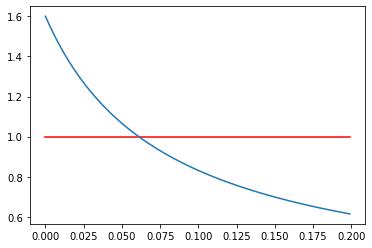
\includegraphics[width=0.5\textwidth]{figures/IMG_ch9/rough.png} % Adjust the width as needed
    \caption{ $(\lambda, \mu) = (1, 0.2)$ in the first phase, and $(\beta, \nu) = (1, 0.9)$. This is the host-to-host GW proliferability measure ($\mean{Z}$) in the BDC to BD case. The plot shows $\mean{Z}$ plotted against $\delta$. What is shown is that for supercritical epidemic spread (under the given assumptions), the initial phase of infection in macrophages should produce a sufficient bacterial load to overcome the likelihood of extinction in only near-supercritical growth in the extracellular phase. This is a consequence of $\delta$ being sufficiently small. That is, the propensity for the macrophage to burst being low permits a higher expected release in this crucial initial phase.}
\end{figure}



\begin{figure}[H]
    \centering
    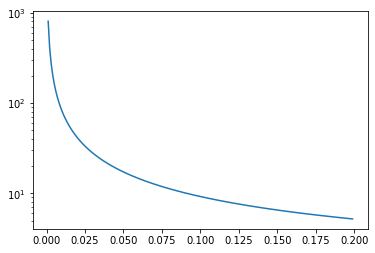
\includegraphics[width=0.45\textwidth]{figures/IMG_ch9/rough2.png}   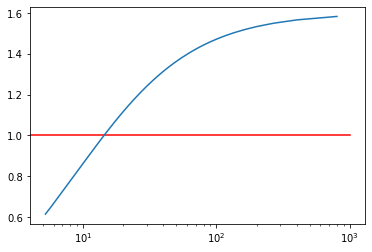
\includegraphics[width=0.45\textwidth]{figures/IMG_ch9/rough3.png} % Adjust the width as needed
    \caption{Left: mean burst size as a function of catastrophe rate $\delta$.  Lower propensity to burst, higher burst size.
Right: GW epidemic replication number $\mean Z$ plotted against mean burst size. High burst size, greater chance of the infection surviving the minimally supercritical pro-inflammatory phase, higher probability of not going extinct, and thus growing exponentially, causing host-to-host proliferation.}
\end{figure}
